\documentclass[12pt]{article}


\usepackage{mathtools}

\usepackage{listings}
\usepackage{xcolor}
\usepackage[english]{babel}
\usepackage[labelfont=bf]{caption}
\captionsetup{labelfont=bf}

\definecolor{codegreen}{rgb}{0,0.6,0}
\definecolor{codegray}{rgb}{0.5,0.5,0.5}
\definecolor{codepurple}{rgb}{0.58,0,0.82}
\definecolor{backcolour}{rgb}{0.95,0.95,0.95}

\lstdefinestyle{mystyle}{
	backgroundcolor=\color{backcolour},   
	commentstyle=\color{codegreen},
	keywordstyle=\color{blue},
	numberstyle=\tiny\color{codegray},
	stringstyle=\color{orange},
	basicstyle=\ttfamily\footnotesize,
	breakatwhitespace=false,         
	breaklines=true,                 
	captionpos=b,                    
	keepspaces=true,                 
	numbers=left,                    
	numbersep=5pt,                  
	showspaces=false,                
	showstringspaces=false,
	showtabs=false,                  
	tabsize=2
}

\lstset{style=mystyle}

\includeonly{
	chapters/introduction,
	chapters/modeling,
	chapters/implementation,
	chapters/verification,
	chapters/simulation_experiments,
	chapters/conclusions
}

\begin{document}


\begin{titlepage}
	\begin{center}
		\begin{figure}
			
\includegraphics[width=\textwidth]{img/marchio_unipi_pant541-eps-converted-to.pdf}         
		\end{figure}
		{\Large
			Computer Engineering\\
			\vspace{5mm} %5mm vertical space
			Performance Evaluation of Computer Systems and Networks}\\
		\vspace{30mm} %5mm vertical space
		{\Huge\textbf{\textit{Slotted random-access wireless network}}}\\
		\vspace{10mm} %5mm vertical space
		{\Large Group Project Report}\\
		\par\noindent\rule{\textwidth}{0.4pt}
		\begin{flushright}
			\textit{TEAM MEMBERS}:\\
			Tommaso Burlon\\ 
			Francesco Iemma\\ 
			Olgerti Xhanej\\
			
		\end{flushright}
		\vfill
		Academic Year: 2020/2021\\        
	\end{center}
\end{titlepage} 
\tableofcontents

\section{Introduction}
\subsection{Problem Description}
From the group project assignment:
\vspace{0.4cm}

\textit{In a \textbf{slotted random-access network}, \textbf{N couples transmitter-receiver} share the same communication
medium, which consists of \textbf{C separate channels}. Multiple attempts to use the same channel in the
same slot by different transmissions will lead to collision, hence no receiver listening on that
channel will be able to decode the message.
Assume that each of the N transmitters generate packets according to an \textbf{exponential interarrival
distribution}, and picks its channel at random on every new transmission. Before sending a packet, it
keeps extracting a value from a \textbf{Bernoullian RV with success probability p} on every slot, until it
achieves success. Then it transmits the packet and starts over. If a collision occurs, then the
transmitter backs off for a random number of slots (see later), and then starts over the whole
Bernoullian experiment.
The number of backoff slots is extracted as $U(1, 2^{x+1})$, where x is the number of collisions
experienced by the packet being transmitted.}
\subsection{Objectives}
The aim of the project report is the \textit{Assessment of the Effectiveness of the Slotted Random-Access Network Protocol} described in the latter paragraph.
\subsection{Performance Indexes}
In order to define a metric of performance of the objective, the following Performance Indexes are defined:
\begin{itemize}
	\item \textbf{Throughput}: let $Tp$ be the Throughput to be measured, $N_{p}$ the number of packets successfully sent in the same timeslot, $T_{timeslot}$ the timeslot duration, the Throughput can be measured as:
	
	\begin{equation}
	Tp = \frac{N_{packets  timeslot}}{T_{timeslot}} = [s^{-1}]
	\end{equation}
	
	\item \textbf{Response Time}: defined as the time that occurs from the first appearance of one packet at the Transmitter up to the reception of the packet at the Receiver.
	\item \textbf{Percentage of Loss Packets}: due to the fact that the transmitter has a limited buffer capacity (see next chapter), there is a need to consider even this variable as a performance index.
	\item \textbf{Network Traffic}: (?)
	\item \textbf{Percentage of Deadlines not respected}: if we consider running this type of communication protocol of a real-time system with his own deadlines, there is a need to consider even this variable as a performance index.
\end{itemize}
% !TeX spellcheck = en_GB
\section{Modeling}
\subsection{Introduction}
The system is modeled as \textbf{N Transmitter-Receiver couples} which communicate through \textbf{C Channels}. A \textit{collision} can occur on a \textbf{Channel} if more than one \textbf{Transmitter} want to transmit a packet in that \textbf{Channel}. The \textbf{Transmitter} stores in a queue the packets that it wants to transmit and, then, it sends them; the \textbf{Channel} "knows" if a collision occurs and handles it; the \textbf{Receiver} only receive packets.  
\subsection{General Assumptions}
The following general assumptions have been made:
\begin{itemize}
	\item \textbf{Slotted}: packets are attempted to be \textbf{Transmitter} by the Transmitter only at the \textbf{beginning of the time-slot}
	\item \textbf{Constant Packet Size and Transmission Rate}: each packet has a \textbf{constant packet size} and each \textbf{Transmitter} has a constant and equal transmission rate for which to transmit a packet (without collision) from the \textbf{Receiver} to the transmitter will last \textbf{one time-slot}.
	\item \textbf{No Propagation Error in the channel}: the only cause of a failed transmission has to be considered the \textit{packet} collision. Other causes, (i.e. path-loss, shadowing, small-scale fading), are neglected. 
	\item \textbf{FIFO Queues of unlimited capacity at the Transmitter} 
	\item \textbf{Transmitters and Receivers always synchronized with the time-slot period}: the \textbf{Receiver} knows in which \textbf{Channel} the \textbf{Transmitter} will try to send his packet in each time-slot and the \textbf{Receiver} will be ready to listen in the correct \textbf{Channel}.
	\item \textbf{After an eventual collision the transmitter will change his channel choice}: this is the default configuration, on Chapter 5 this configuration will be compared with the Non-Change Channel one.
\end{itemize}

\subsection{Preliminar Validation}
Before the implementation a preliminar validation phase is necessary to ensure that the model is correct. Let analyze if the assumptions made in the previous section are reasonable:
\begin{itemize}
	\item The \textbf{slotted assumption} (transmission only at the beginning of the timeslot) is reasonable due to the fact that exist some network protocols which work under this assumption, see for instance Slotted Aloha. % \colorbox{yellow}{that is the most famous one}.
	\item We consider the \textbf{packet size constant} because if the packet length is so large that more than one slots are needed, we can consider, from the viewpoint of the model, that this unique packet send in two different slots is like two packets of fixed-length send each one in a slot. Taken this into account is reasonable to state that the packet size is constant and that one packet is transmitted within a slot (if no collisions occur).
	\item The critical issue of every slotted network is the one related to the \textbf{collisions}: they have an huge impact on the general performance of the network, so it is reasonable to neglect the other propagation errors that are not network-specific or that depend from the environment (as path-loss).
	\item It's reasonable that the transmitter and the receiver are \textbf{synchronized with the time-slot period}, in fact other slotted-based network as slotted ALOHA requires a synchronization of this type.
	%\item \colorbox{yellow}{When a packet collide it's reasonable} to think that the transmitter will change the transmission channel in order to avoid another collision. Indeed this along with the back-off time are the techniques that should avoid another collision. 
\end{itemize}
\subsection{Factors}
The following factors have been defined which may affect the performance of the system:
\begin{itemize}
	\item \textbf{N}: \textbf{Transmitter-Receiver} Couples.
	\item \textbf{C}: numbers of \textbf{Channels}.
	\item \textbf{p}: \textbf{probability of success} for sending a packet in the current time-slot for a Transmitter.
	\item \textbf{$\dfrac{1}{\lambda}$}: exponential distribution \textbf{mean inter-arrival time of packets} at the Transmitter.
	\item $T_{slot}$: \textbf{time-slot duration}.
	
\end{itemize}
\section{Implementation}
\subsection{Modules}
The following modules have been defined:
\begin{itemize}
	\item \textbf{Transmitter}: duty of sending a packet to a specific channel.% Parameters: $lambda$, $p$, packetsInQueue Signal (for the queue)
	\item \textbf{Channel}: duty of checking every channel in each timeslot for any collision.% Parameters: $T_{timeslot}$, Throughput Signal
	\item \textbf{Receiver}: duty of receiving a packet from the channel.
\end{itemize}

\begin{figure}[H]
	\centering
	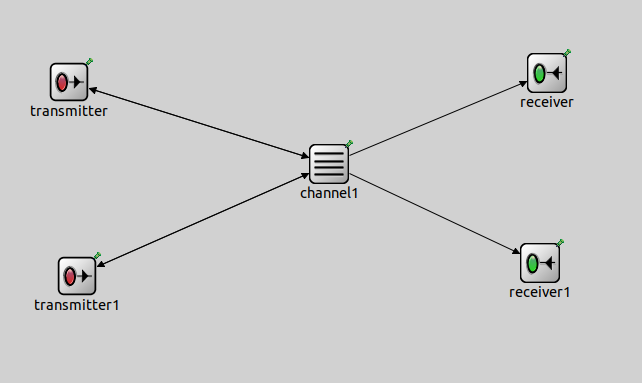
\includegraphics[width=0.6\textwidth]{img/network.png}
	\caption{Network example}
	\label {img: network}
\end{figure}

\subsection{Messages}
A new format of message has been defined, in order to store all packet information, with the following fields:
\begin{itemize}
	\item \textit{simtime$\_$t creationTime}: time in which the packet arrives for the first time at the \textbf{Transmitter}
	\item \textit{int idChannel}: \textbf{Channel} chosen for the current transmission, may change in case of collision
	\item \textit{int idTransmitter}: Id of the module \textbf{Transmitter} that has sent the message
	\item \textit{int idGate}: Id of the gate in which the \textbf{Transmitter} is linked to the \textbf{Channel}
\end{itemize}

\subsection{Modules Behaviour}
\subsubsection{\textit{Transmitter} Module Behaviour in the implementation}
\begin{enumerate}
	\item Message arrival at the \textit{Transmitter}:
	\begin{itemize}
		\item \textbf{IF} an \textit{ACK} has been received, the packet at the top of the queue can be removed. \textbf{GOTO (2)}
		\item \textbf{ELSE IF} a \textit{NACK} has been received, then the \textit{Transmitter} starts his backoff time and \textbf{waits for another message}.
		\item \textbf{ELSE IF} a \textit{Synchronization message} has been received \textbf{AND} the \textit{Transmitter} is not in backoff-time \textbf{GOTO (2)}
		\item \textbf{ELSE IF} a \textit{packet} arrives at the \textit{Transmitter}, the \textit{Transmitter} stores the packet in the queue, make a reschedule of the arrival of the next packet and \textbf{waits for another message}
	\end{itemize}
	\item The \textit{Transmitter} tries to send the packet
	\begin{itemize}
		\item \textbf{IF} success on the Bernoullian Experiment, then the packet will be forwarded to the \textit{Channel}.
		\item \textbf{ELSE waits for another message}
	\end{itemize}
\end{enumerate}
\subsubsection{\textit{Channel} Module Behaviour in the implementation}
\begin{enumerate}
	\item The \textit{Channel} wakes up at the beginning of each time slot and checks his channels status.
	\begin{itemize}
		\item \textbf{IF} two or more packets have arrived in the same channel, the \textit{Channel} will send a NACK to the \textit{Transmitters} that have forwarded the packets in that specific channel.
		\item \textbf{ELSE IF} one and only one packet has arrived in a channel, the \textit{Channel} will send an ACK to the relative \textit{Transmitter} and will forward the packet to the \textit{Receiver}.
		\item \textbf{ELSE} the \textit{Transmitters} that did not send a packet will receive from the Channel a \textit{Synchronization Message}
	\end{itemize}
	\item The \textit{Channel} will gather of the packets for the current time slot, to be processed in the next one. So this means that if the channel receives packets in time-slot \emph{j}, then the information about collisions are provided to transmitters in time-slot \emph{j+1}. Hence, from the point of view of the transmitter, the information received at \emph{j+1} are referred to events took place in \emph{j}.
\end{enumerate}
\subsubsection{\textit{Receiver} Module Behaviour in the implementation:}
\begin{enumerate}
	\item The \textit{Receiver} wakes up when a packet arrives. Due to the fact that the receiver essentially has the only duty of receiving packets. It computes statistics on the number of packets received mainly for debugging purpose.
\end{enumerate}
% !TeX spellcheck = en_GB
\section{Verification}
In this section we present tests performed in order to verify that our implementation reflects correctly our model.

\subsection{Degeneracy Tests}
In the degeneracy tests we verify the behaviour of our simulator with parameters set to 0 values. In all tests the simulator works properly. In particular the following observations can be inferred:
\begin{itemize}
	\item If the number of channel is 0 then the simulation stops immediately because has no sense running a simulation with 0 channels.
	\item If the time slot size is 0 then the simulation doesn't stop and goes to infinite because on instant 0  time slots are continuously triggered.
	\item If the exponential mean is 0 then the simulation doesn't stop and continues to infinite because packets arrive at time 0 continuously.
\end{itemize}

\subsection{Consistency Test}
The consistency test verifies that the system react consistently with the output. In order to test this we perform two tests with the following parameters.
\paragraph{Test 1}
\begin{itemize}
	\item Number of couple tx-rx: 1
	\item Number of channels: 500
	\item Send probability: 1
	\item Mean inter-arrival time: 10s (deterministic)
	\item Time slot size: 5s
\end{itemize}

\paragraph{Test 2: Two couple TX-RX with half packets arrival rate}
\begin{itemize}
	\item Number of couple tx-rx: 2
	\item Number of channels: 500
	\item Send probability: 1
	\item Mean inter-arrival time: 20s (deterministic)
	\item Time slot size: 5s
\end{itemize}

\noindent We expect that the result of the two tests are more or less equal because the behaviour of one source transmitting every 10 seconds must be similar to the behaviour of two sources transmitting every 20 seconds. We set the number of channels at 500 in order to neglect the effect of collisions (in any case it is possible that a collision occur, but in the following tests no collisions have been detected).

\noindent The graph in figure \ref{img: consistencyTest1a} and in figure \ref{img: consistencyTest1b} show the results of the tests previously explained. We can see that the behaviour is very similar in both cases and so that the systems works as we expect. In fact the Mean Throughput per slot tend in both cases to 0.50 packets per slot.

\begin{figure}[H]
	\centering
	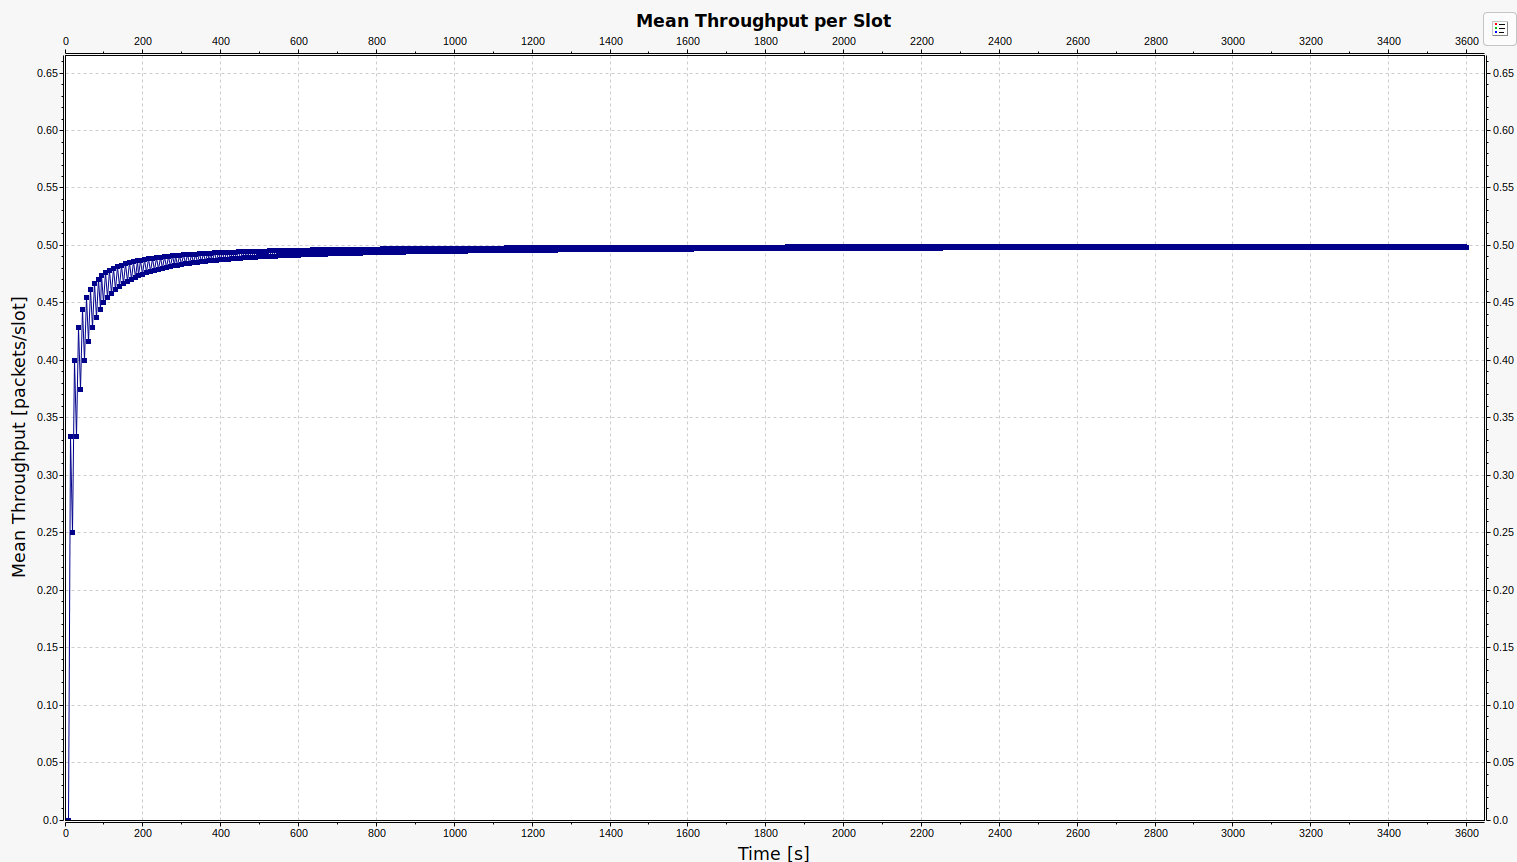
\includegraphics[width=0.9\textwidth]{img/consistencyTest1aWithAxis.png}
	\caption{Consistency Test 1}
	\label {img: consistencyTest1a}
\end{figure}

\begin{figure}[H]
	\centering
	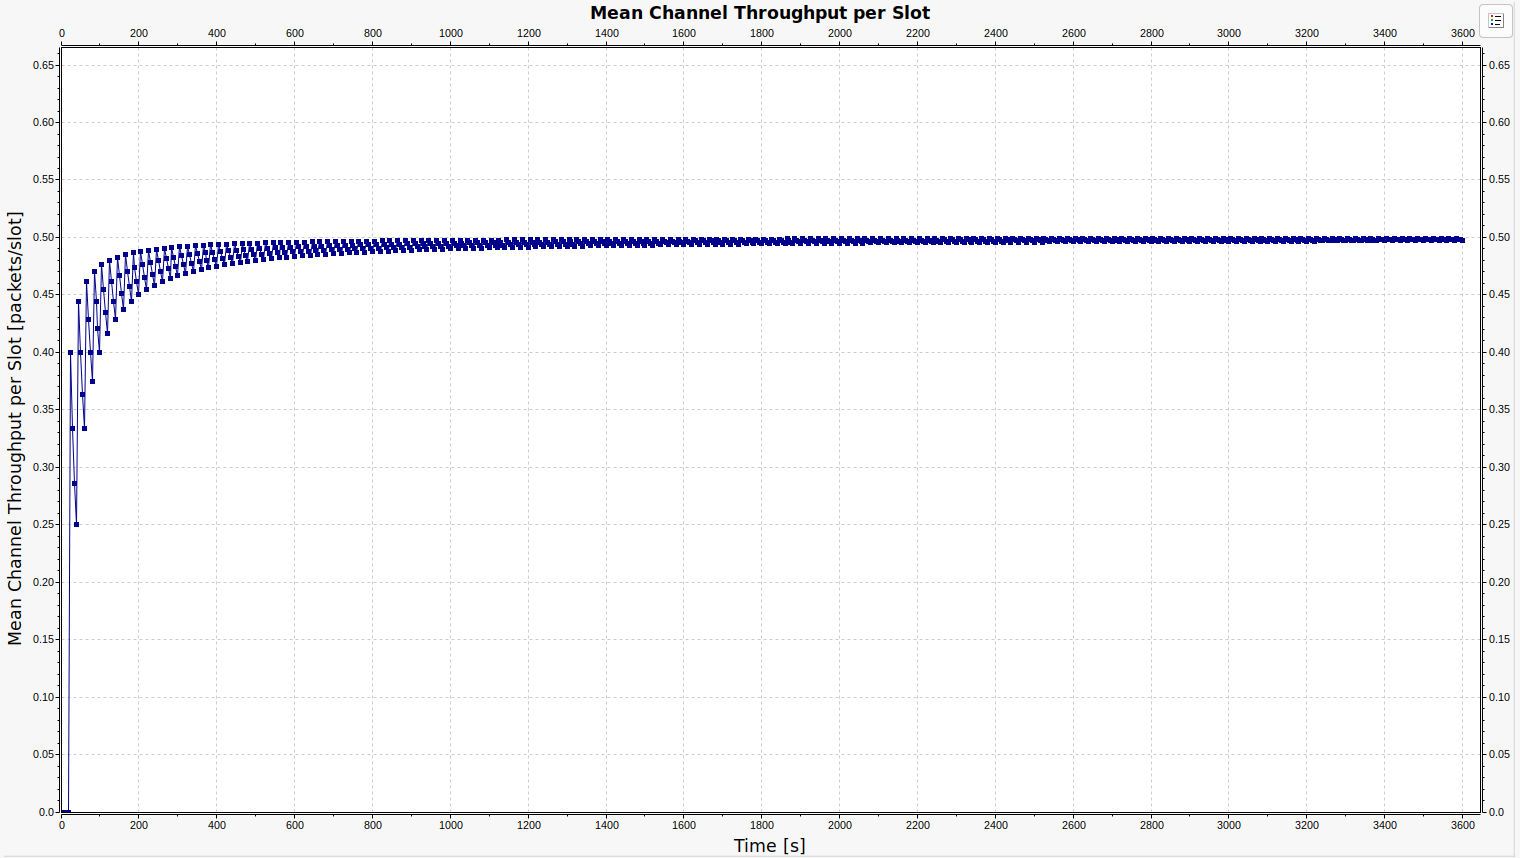
\includegraphics[width=0.9\textwidth]{img/consistencyTest1bWithAxis.png}
	\caption{Consistency Test 2}
	\label {img: consistencyTest1b}
\end{figure}

\noindent The oscillations at the beginning are due to the fact that the mean inter-arrival time is bigger with respect to the time slot size. In fact we can observe that in the second test there are larger oscillations because the difference between the mean inter-arrival time and the time slot size is bigger than the one of the first test.

\noindent Now let analyse the response time, we can see its measure in both tests in figure \ref{img: consistencyTest1a_responsetime} and \ref{img: consistencyTest1b_responsetime}.

\begin{figure}[H]
	\centering
	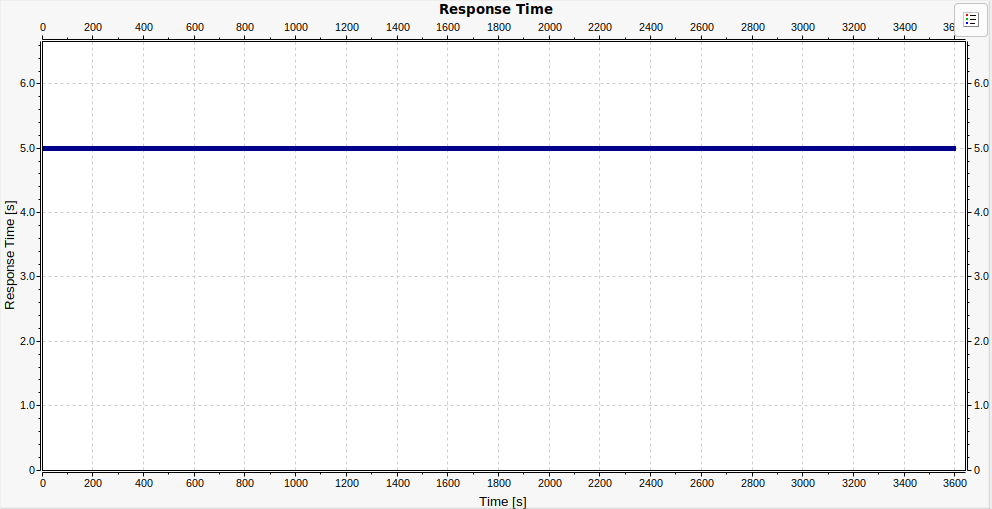
\includegraphics[width=0.9\textwidth]{img/consistencytest1a_responsetime.png}
	\caption{Consistency Test 2 - Response Time}
	\label {img: consistencyTest1a_responsetime}
\end{figure}

\begin{figure}[H]
	\centering
	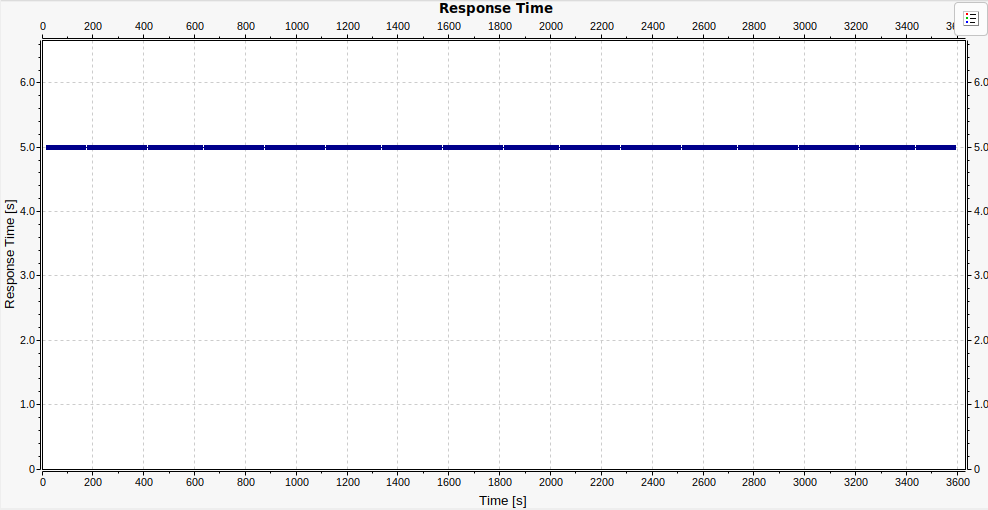
\includegraphics[width=0.9\textwidth]{img/consistencytest1b_responsetime.png}
	\caption{Consistency Test 2 - Response Time}
	\label {img: consistencyTest1b_responsetime}
\end{figure}


\noindent The mean response time in both cases is 5 seconds, this is a lower bound for the response time because in both tests 5 seconds is the size of the slot time so it's impossible to have a response time lower than the slot size.

\noindent We can see that in the second test we have a less continue plot, this is due to the fact that the mean inter-arrival time is bigger in the second case and so the packet are more distant in time.

\noindent We can conclude that also for what concerns the response time the consistency is ensured because it is the same in the case in which we have a source transmitting each 10 seconds and in the case in which we have two sources transmitting each 20 seconds. 

\subsection{Continuity Test}
In this test the aim is to prove that the output changes slightly if the input changes a bit. In order to do prove this, 2 simulations have been performed with the parameters shown in table \ref{tab: continuity test}. With this parameters we have changed slightly the input, and so we expect that the outputs don't show particular differences. Obviously some differences will be present (in particular due to collisions and the increasing in the number of transmitters) but they shouldn't affect a lot the results.

\begin{table}[htpb]
	\centering
		\begin{tabular}{|c|c|c|ll}
			\cline{1-3}
			{\textbf{Test}} & { \textbf{Number of Transmitters}} & { \textbf{Number of Channels}} &  &  \\ \cline{1-3}
			1 & 8  & 20 &  &  \\ \cline{1-3}
			2 & 10 & 20 &  &  \\ \cline{1-3}
		\end{tabular}
	\caption{Continuity test parameters}
	\label{tab: continuity test}
\end{table}

\noindent The remaining parameters are the same of all of four tests:
\begin{itemize}
	\item Send probability: 1
	\item Mean Inter-arrival time: 10 sec (deterministic)
	\item Time slot size: 5 sec
	\item Threshold: 20 sec
\end{itemize}

\noindent The results of the simulation as shown in the figure \ref{img: continuityTest1a} and \ref{img: continuityTest1b} (we measure the mean throughput).

\begin{figure}[H]
	\centering
	\includegraphics[width=0.8\textwidth]{img/continuityTest1a.png}
	\caption{Continuity Test 1 - Mean Throughput per Slot - Collisions detected: 272}
	\label {img: continuityTest1a}
\end{figure}

\begin{figure}[H]
	\centering
	\includegraphics[width=0.8\textwidth]{img/continuityTest1b.png}
	\caption{Continuity Test 2 - Mean Throughput per Slot - Collisions detected: 390}
	\label {img: continuityTest1b}
\end{figure}

\noindent We can observe that the output changes slightly between the two cases. In particular it's possible to infer that if the number of transmitter increases then the throughput increases too, but this increasing is reduced by the collisions, in fact if the number of channels is fixed, the more the transmitter the more the collisions.

\noindent At the end of the day we can see that in the first case the mean throughput is settled to a value about 3.6 and in the second case about 4. So changing slightly the input changes slightly the output.

\noindent If we analyze the response time we can see that the difference is bigger between the two cases because the response time is sensible to the variation of transmitters and channels, and this is something that must be taken into account. In fact, as we have seen previously, there are a lot of collisions in the second case and this is the main reason for the increasing of response time in the second test w.r.t the first one.



\begin{figure}[H]
	\centering
	\includegraphics[width=0.8\textwidth]{img/continuityTest1a_responsetime.png}
	\caption{Continuity Test 1 - Response Time - Collisions detected: 272}
	\label {img: continuityTest1a_responsetime}
\end{figure}

\begin{figure}[H]
	\centering
	\includegraphics[width=0.8\textwidth]{img/continuityTest1b_responsetime.png}
	\caption{Continuity Test 2 - Response Time - Collisions detected: 390}
	\label {img: continuityTest1b_responsetime}
\end{figure}

\noindent It's possible to see the response time measured in the two tests in the figure \ref{img: continuityTest1a_responsetime} and \ref{img: continuityTest1b_responsetime}. In any case we can see that the continuity test is correct because the system works as we expect: channels fixed, the more the transmitters, the more the collisions, the more the response time.

\vspace{5mm}
In addition to this, some simulation were taken in order to \textbf{assess the monotonicity} of some KPI by changing some factors:
\begin{itemize}
	\item \textbf{Mean Throughput}: By \textbf{increasing N} (the numbers of couples tx-rx), with a high number of channels to avoid collisions, an \textbf{increase on the mean throughput is expected}. On the contrary, by \textbf{increasing} $\dfrac{1}{\lambda}$ (the mean inter-arrival time) an \textbf{opposite result is expected}. The following results were obtained:
	\begin{figure}[H]
		\centering
		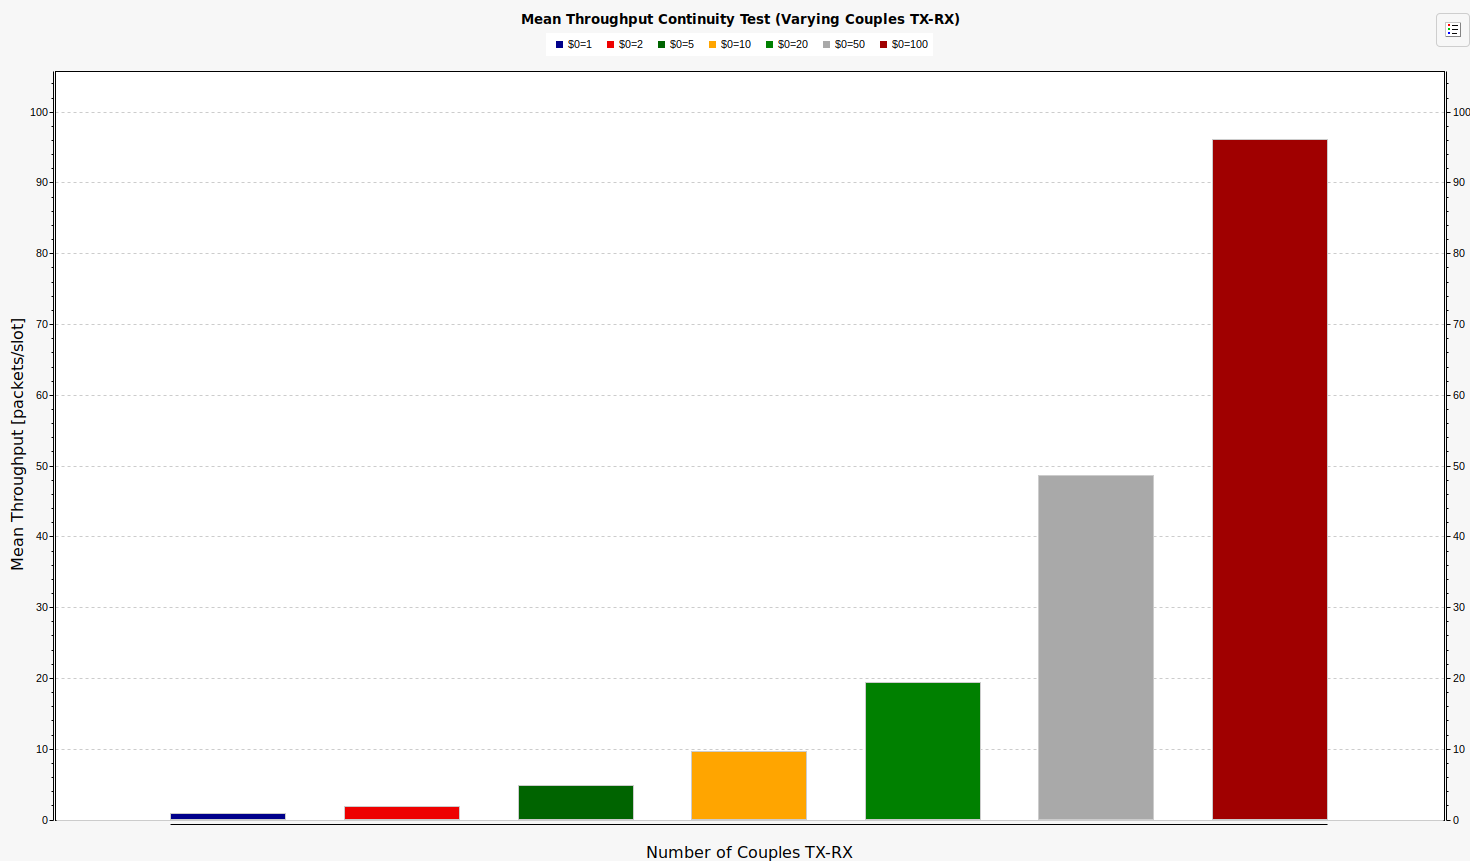
\includegraphics[width=\textwidth]{img/continuityTest_Throughput_TXRX_Varying.png}
		\caption{Continuity Test - Increasing Number of TX-RX (Main factors: \textbf{N} = 1, 2, 5, 10, 20, 100; \textbf{C} = 20000; $\dfrac{1}{\lambda}$ = 20 ms; $T_{slot}$ = 5ms; $p$ = 1)}
		\label {img: continuityTestThTXRX}
	\end{figure}
	\begin{figure}[H]
		\centering
		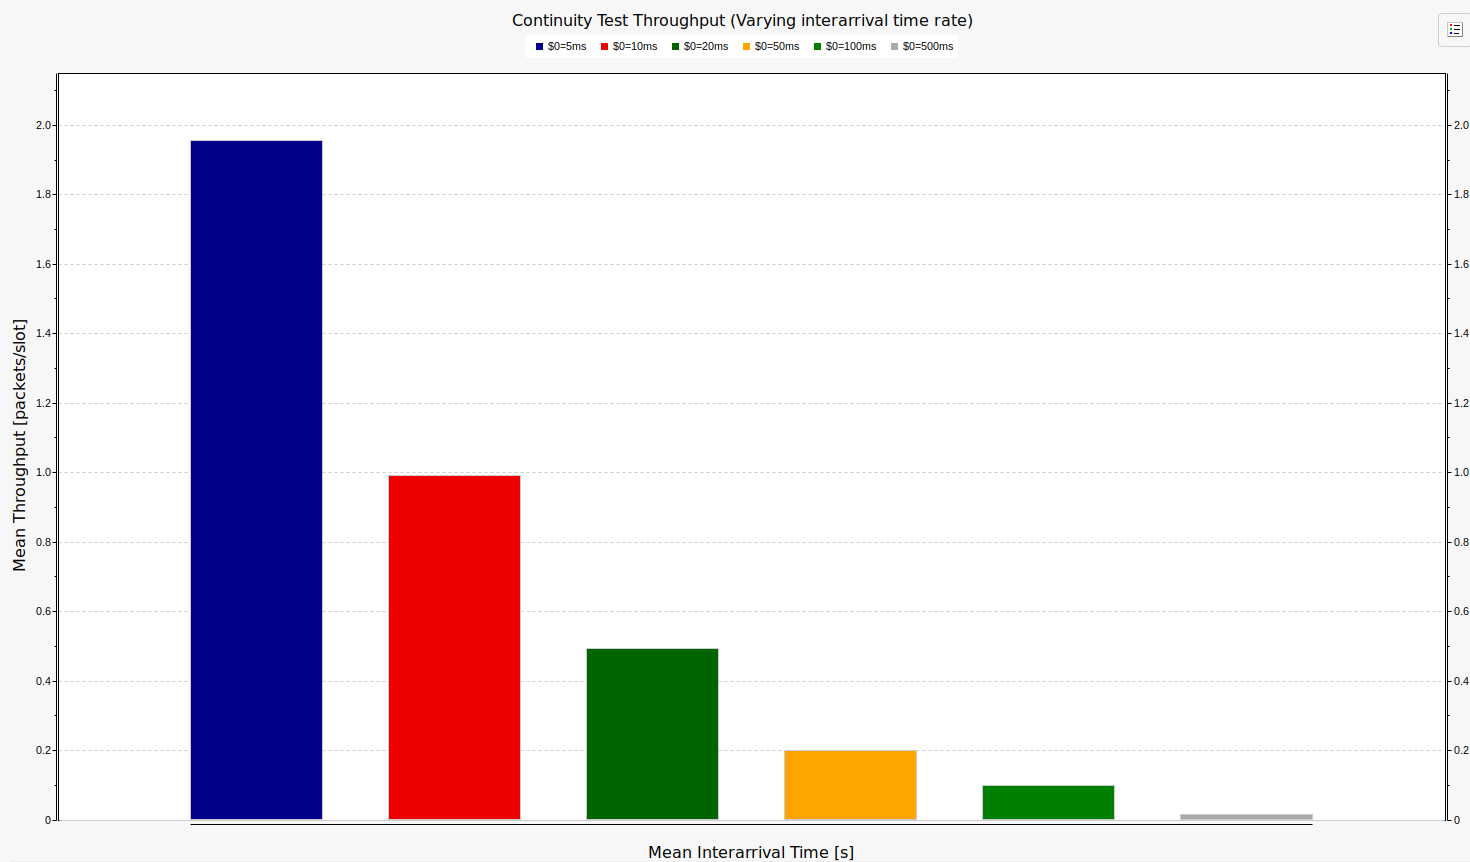
\includegraphics[width=\textwidth]{img/continuityTest_Throughput_IntTimeVarying.png}
		\caption{Continuity Test - Increasing Mean Inter-arrival Time (Main factors: \textbf{N} = 2; \textbf{C} = 20000; $\dfrac{1}{\lambda}$ = 5ms, 10ms, 20ms, 50ms, 100ms, 500ms; $T_{slot}$ = 5ms; $p$ = 1)}
		\label {img: continuityTestThLambda}
	\end{figure}
	\item \textbf{Mean Response Time}: By \textbf{Increasing N} ()the number of couples tx-rx), with low numbers of channels, a \textbf{increase on the mean response time is expected}. By increasing the transmission probability $p$ (with a low number of couples tx-rx) a decrease on the mean response time is expected due to more transmissions. The following results were obtained:
	\begin{figure}[H]
		\centering
		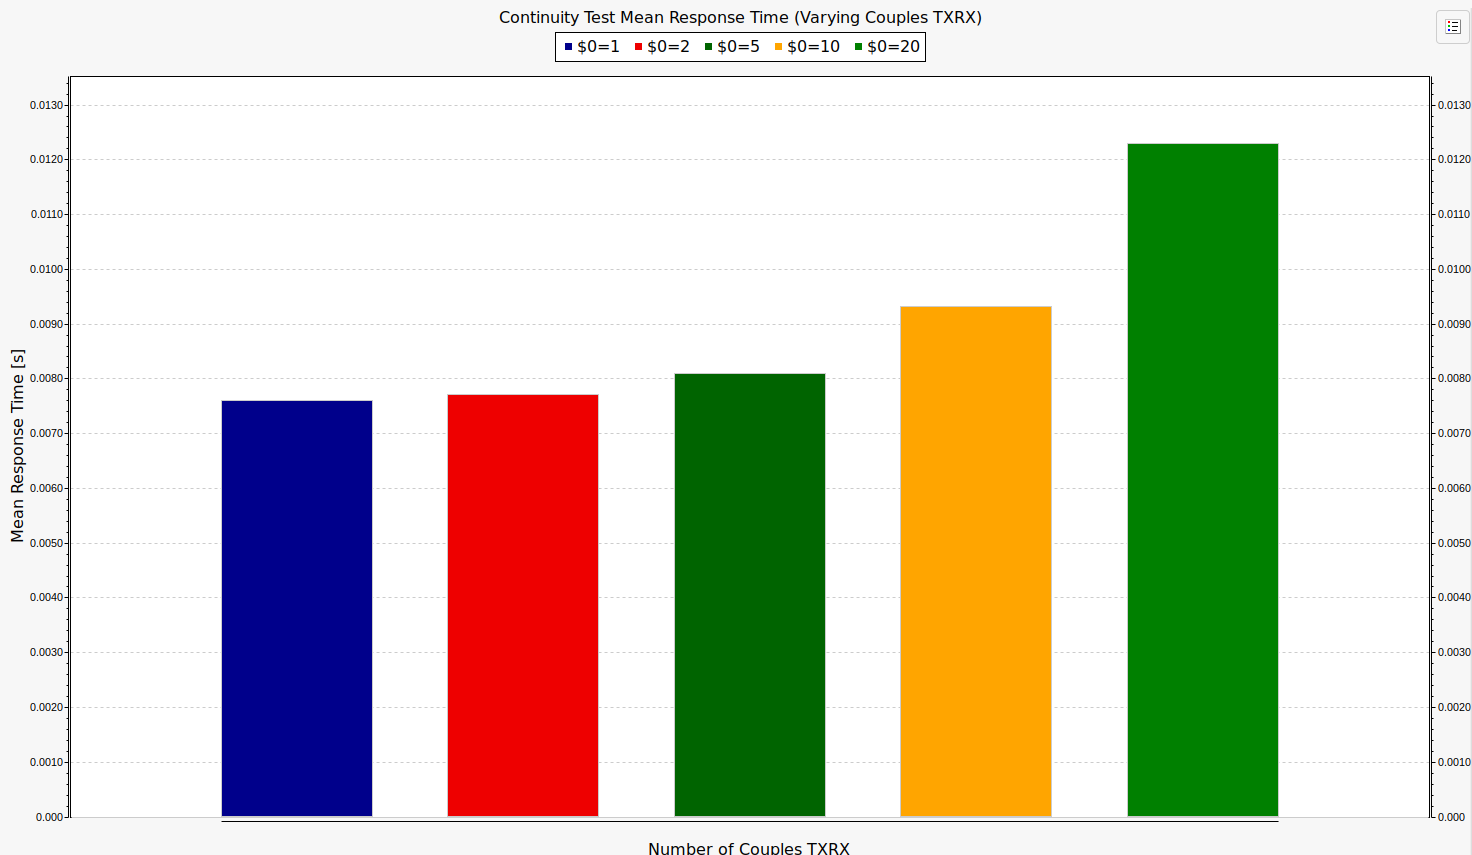
\includegraphics[width=\textwidth]{img/ContinuityTest_ResponseTIme_TXRXVarying}
		\caption{Continuity Test Mean Response Time- Increasing Number of TX-RX}
		\label {img: continuityTestTXRXResponse}
	\end{figure}
	\begin{figure}[H]
		\centering
		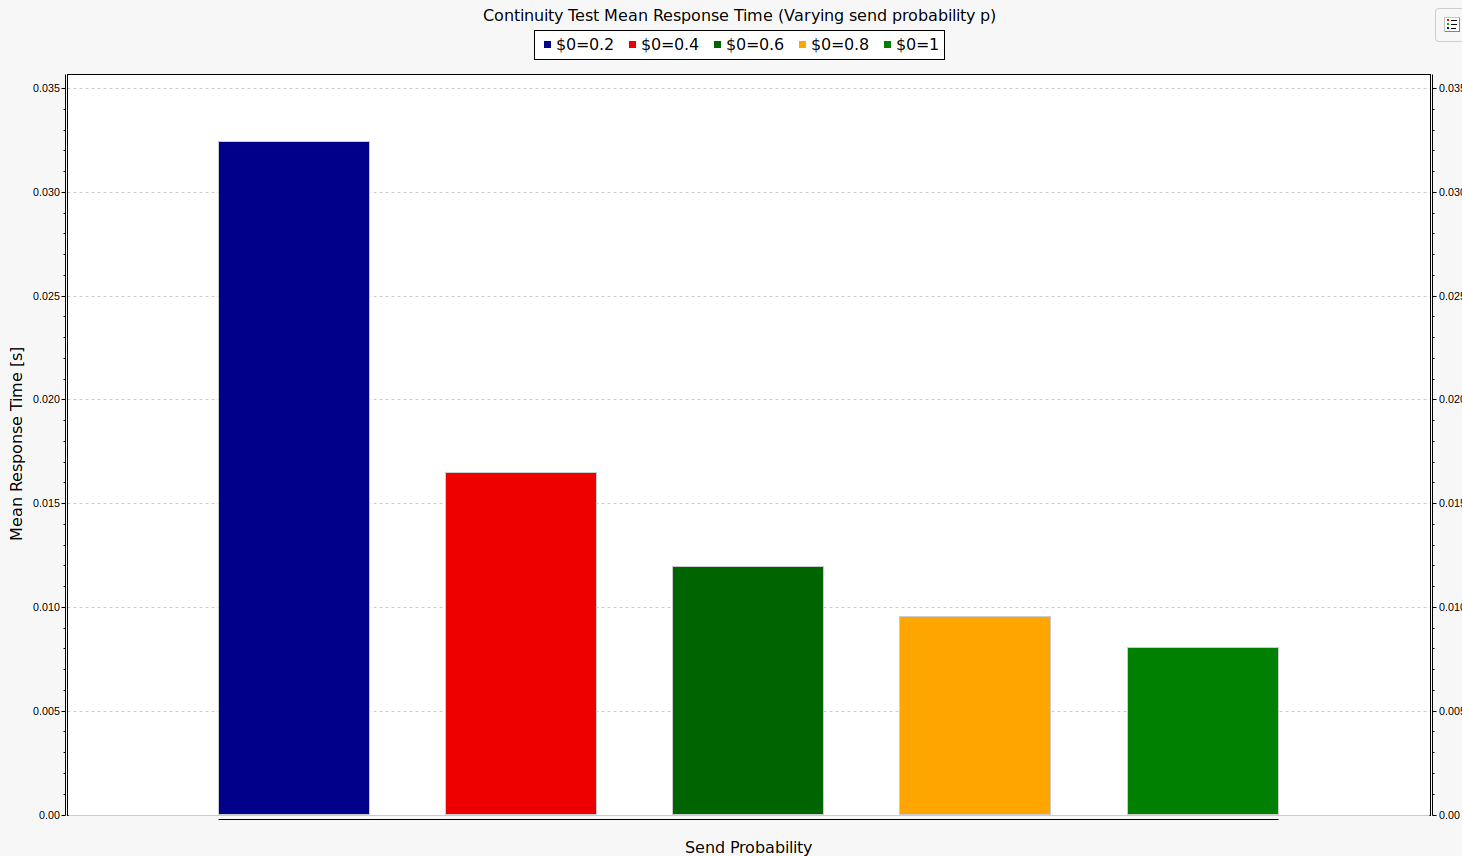
\includegraphics[width=\textwidth]{img/ContinuityTest_ResponseTIme_VaryingP.png}
		\caption{Continuity Test Mean Response Time- Increasing Sending Probability P(Main factors: \textbf{N} = 5; \textbf{C} = 4; $\dfrac{1}{\lambda}$ = 200ms; $T_{slot}$ = 5ms; $p$ = 0.2, 0.4, 0.6, 0.8, 1)}
		\label {img: continuityTestResponseLambda}
	\end{figure}
\end{itemize} 
\textbf{For the Mean Response Time was also checked the steady state reach} by just plotting that the relative vector stabilizes at some point (this was done in general to make conclusion with this KPI). Here an example for the varying of the Transmission Probability $p$:
\begin{figure}[H]
	\centering
	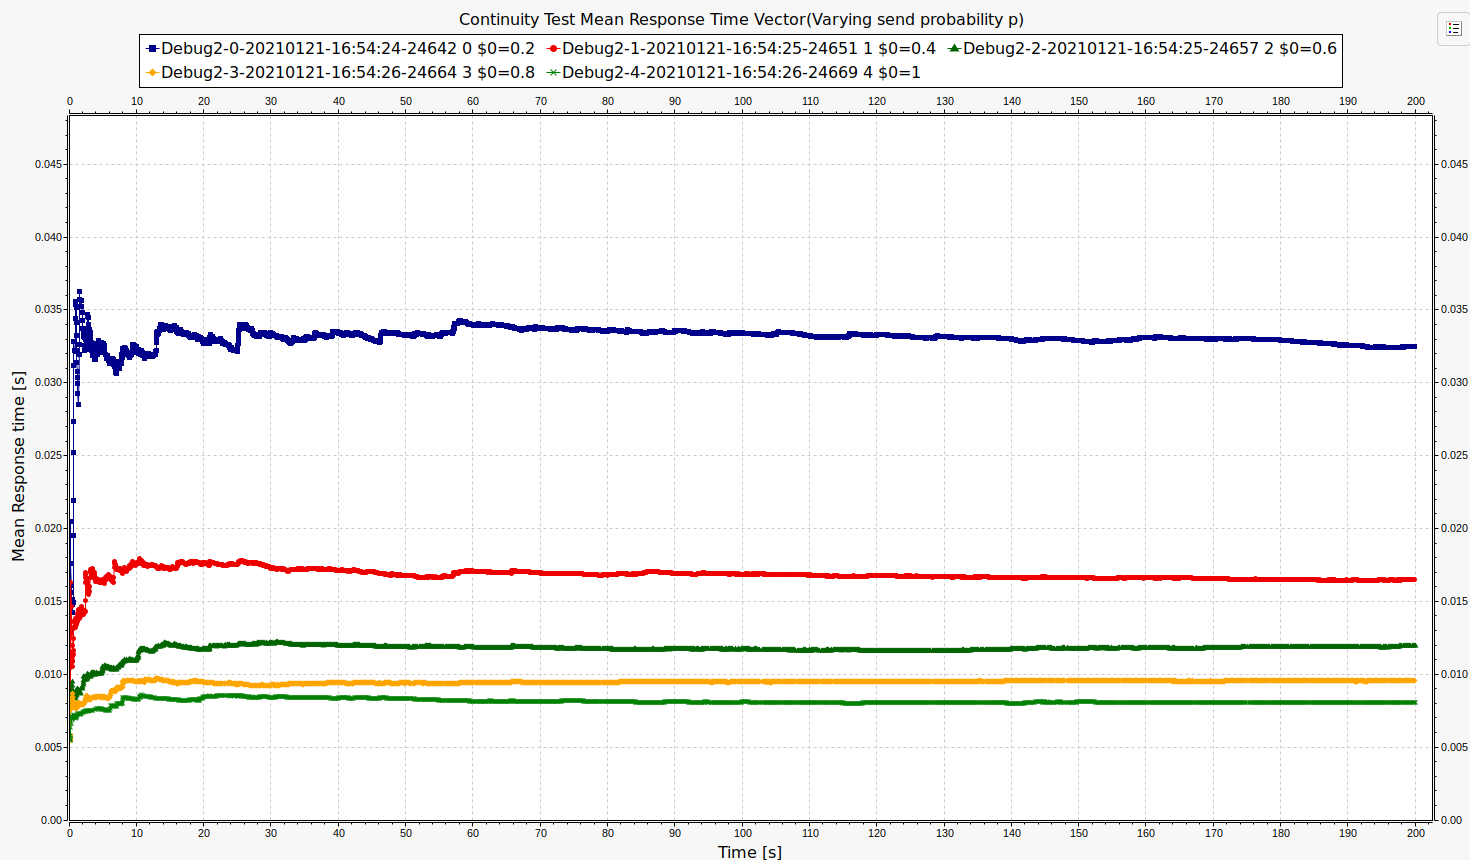
\includegraphics[width=0.8\textwidth]{img/ContinuityTest_ResponseTime_VectorP.png}
	\label {img: responseTimeConvergence}
\end{figure}
\subsection{Test Simulations with Binomial Model (1)}
This test simulation has been performed with the following parameters:
\paragraph{Parameters}
\begin{itemize}
	\item Number of couple tx-rx: 1
	\item Number of channels: 1
	\item Send probability: \$\{0.2, 0.4, 0.5, 0.6, 0.8\} ($p$)
	\item Mean inter-arrival time: 1s (deterministic) ($lambda$)
	\item Time slot size: 2s ($T_{slot}$)
	\item simulation-duration: 3600s ($T_{sim}$)
	\item repeat: 100
	\item seed-set: \$\{repetition\}
\end{itemize}
In this simplified context there are no collisions (only one couple) and the transmitter will have, for every slot, at least one packet to sent ($lambda < T_{slot}$). We can model this particular case as a repeated Bernoullian Experiment, in which a success event correspond to a successful packet sent. In this simplified model we can define X as the number of success in n repeated trials (in independent condition), so $X \sim Bin(n, p)$. For this reason the PMF is the following:
\begin{equation}
	p(i) = P\{X = i\} = \binom{n}{i} p^{i} (1-p)^{n-i}
\end{equation}
Where $n$ represents the number of repeated trials and $i$ the number of successes in those trials. With this distribution the mean and the variance are:
\begin{align*}
	E[X] = np \qquad     
	Var(X) = np(1-p)
\end{align*}
In our context we can state the following:
\begin{equation}
	n = \left \lfloor{\dfrac{T_{slot}}{T_{sim}}}\right \rfloor = 1800
\end{equation}
We would expect in the case of $p = 0.5$:
\begin{equation}
	E[X] = np = 900
\end{equation}
And the results after the run of 100 test simulation with different seeds, the following results are returned (with 95\% CI):
\begin{equation}
	\overline{X} \in [893.08, 901.94]
\end{equation}
Which is in line with our expectations. The latter computations have been repeated for different values of p and the following plot can sum up the results:

\begin{figure}[H]
	\centering
	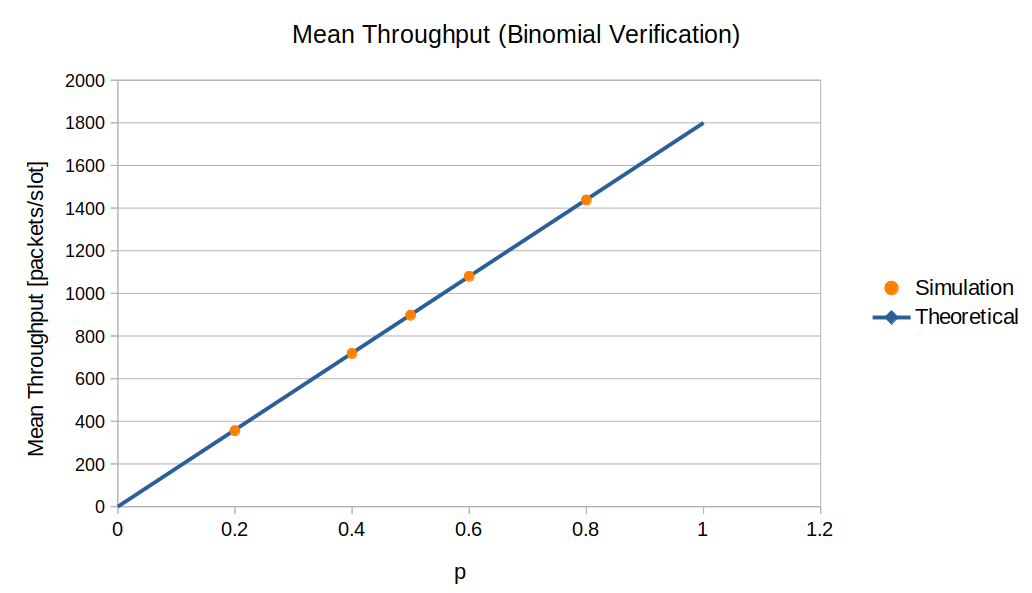
\includegraphics[width=0.9\textwidth]{img/plotTheoreticalMeanBinomial.png}
	\caption{Test Binomial Model}
\end{figure}

As we can see it is difficult to recognize the theoretical results with the results obtained with the test simulations and the Confidence Interval can be barely seen.

\subsection{Test Simulations with Collisions(2)}
This test simulation has been performed with the following parameters:
\paragraph{Parameters}
\begin{itemize}
	\item Number of couple tx-rx (N): \$\{2, 5, 10, 30\}
	\item Number of channels (C): 1
	\item Send probability: \$\{0.2, 0.4, 0.6, 0.8\} ($p$)
	\item Mean inter-arrival time: 1s (deterministic) ($lambda$)
	\item Time slot size: 2s ($T_{slot}$)
	\item simulation-duration: 3600s ($T_{sim}$)
	\item repeat: 40
	\item seed-set: \$\{repetition\}
	\item No Backoff in case of collision
\end{itemize}

\noindent The aim of this verification is to assess if the mean throughput is comparable with some equations that will be found even in the case of presence of collisions. \\

\noindent The probability of a successful sent in a particular timeslot, in this case, is the following:
\begin{equation}
	P\{" successful\ transmission"\} = P\{"only\ one\ tx\ transmit"\} = Np(1-p)^{N-1}
\end{equation}

Note that the above case is equal to the case without collisions.

By comparing the above formula with the results of the simulation the following results are obtained (95\% CI too small to be seen)
\begin{figure}[H]
	\centering
	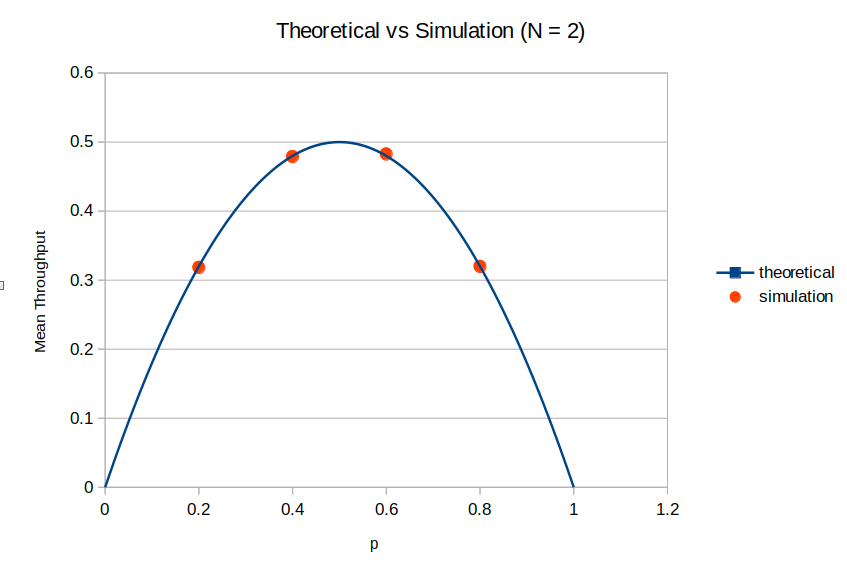
\includegraphics[width=\textwidth]{img/SecondVerificationN2.png}
\end{figure}
\begin{figure}[H]
	\centering
	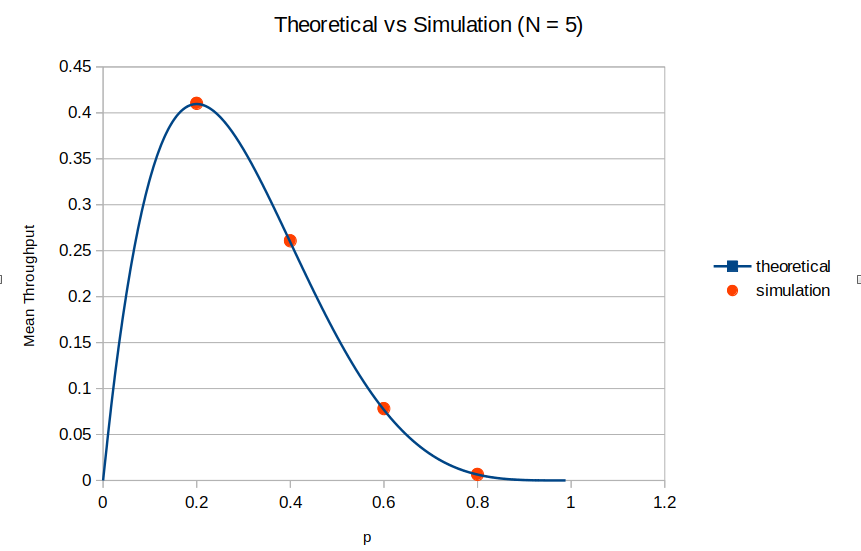
\includegraphics[width=\textwidth]{img/SecondVerificationN5.png}
\end{figure}
\begin{figure}[H]
	\centering
	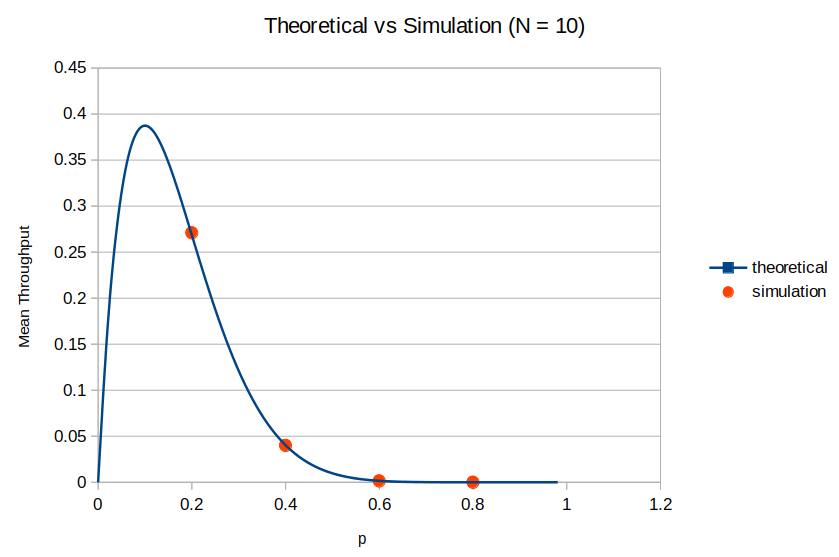
\includegraphics[width=\textwidth]{img/SecondVerificationN10.png}
\end{figure}
\begin{figure}[H]
	\centering
	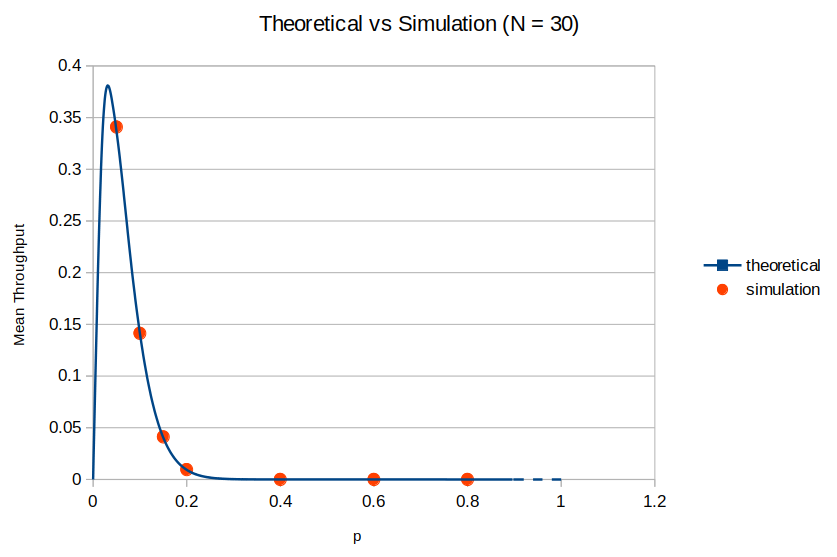
\includegraphics[width=\textwidth]{img/SecondVerificationN30.png}
\end{figure}

At this point we can state that a proper amount of verification of the implementation of the model has been carried out to make some simulation and gather some insight. Before doing so, an observation of the result can be carried out at this point: with a good number of couple tx-rx a huge sending probability (i.e. greater than 0.5) is pointless to obtain a high throughput. This result will be considered during the scenario calibration in the next chapter. 
\section{Simulations Experiments}
\subsection{Scenario Calibration}
In order to calibrate the simulator parameters, the following range of values were used:
\begin{itemize}
	\item \textbf{Number of Couples Tx-Rx}: [5, 30]
	\item \textbf{Number of Channels C} : [6, 100] (Resource Blocks in LTE for different Frequencies)
	\item \textbf{Mean Inter-arrival Time (1/lambda)}: [25ms, 500ms]   
	\item \textbf{Time-slot duration $T_{slot}$}: 0.5 ms (Timeslot duration in LTE)
	\item \textbf{Time Threshold}: [5ms, 50ms] 
	\item \textbf{Send Probability p}: [0.2, 0.5] 
\end{itemize}

\subsection{Calibration of Warm-Up Period and Simulation duration}
For calibrating the warm-up different simulation were made (with the factors range in the latter paragraph) with 10 repetition each. 
The worst case in terms of convergence time was encountered with the \textbf{mean throughput} with N = 5, C = 6, $\dfrac{1}{\lambda}$ = 500ms, p = 0.5:
\begin{figure}[H]
	\centering
	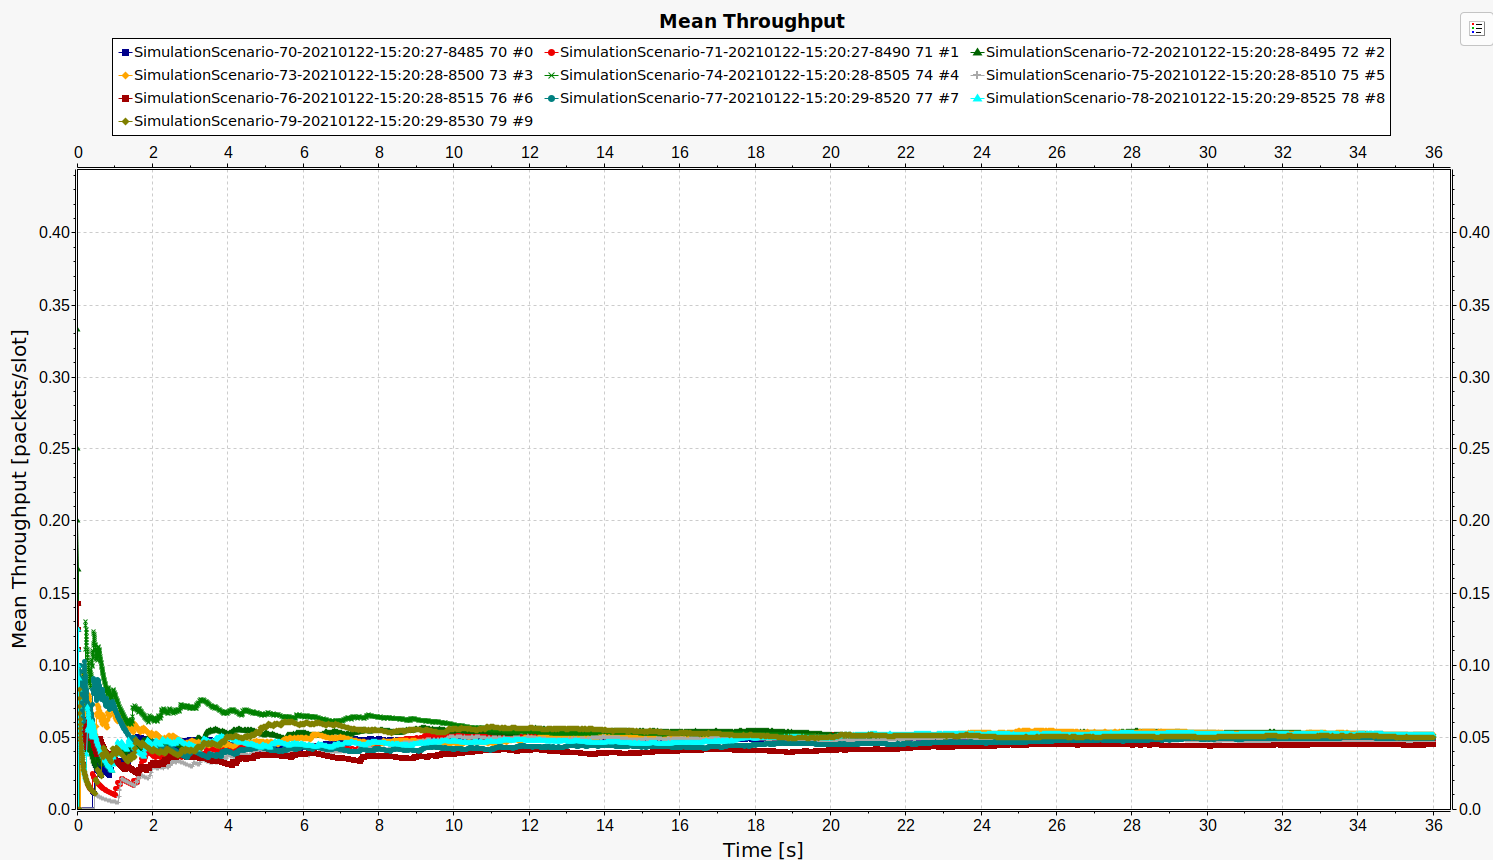
\includegraphics[width=\textwidth]{img/WorstCaseWarmUp.png}
	\caption{Worst Case Warm-up}
	\label {img: warmUp}
\end{figure}  
\noindent\textbf{A warm-up period of 10s was chosen}.
For what concerns the simulation duration was made a trade-off between the memory consumption and the length of the simulation itself. This was done because there are not stochastic elements in the model (like a particular error probability with a low percentage) that will need a particular amount of time to be shown. Obviously the duration has to be greater than the warm-up duration. All things considered, \textbf{a simulation-duration of 100s was chose}

\subsection{Design of Experiments}
\subsection{Result Analysis}
% !TeX spellcheck = en_GB
\section{Conclusions}
The final consequences of the report are shown in this section. 
The results obtained in the \textbf{Response Time Explosion scenario} underlines \textbf{three aspects}:
\begin{itemize}
	\item The \textbf{No-Change of channel sub-scenario} (in case of collision), is \textbf{worst in terms of throughput} than the Change Channel one, \textbf{when the number of trasmitters start to grow} (so more collisions expected mantaining fixed the number of channels that will makes more clear the difference between the two scenarios)
	\item An \textbf{higher Send Probability is better} in this case because \textbf{maximizes the throughput} (consideration on Response Time can't be done). This increase start grows faster at the beginning of the increase of p. 
	\item The \textbf{Throughput keeps increasing with the number of Transmitters} (with our ranges) and is the \textbf{most relevant factor} as underlined in the relative $2^{k}r$ experiment.
\end{itemize} 
%Considering the join effect of the KPIs we can say that the Slotted Random-Access Wireless Network studied has good performance and the following observations about it can be done. 

\noindent %As first observation we can say that the system is fair. We can say this due to the Lorenz Curve (figure \ref{img: insight2_throughput}, \ref{img: insight2_respTime}, \ref{img: insight3_respTime}).

\noindent Moreover the overall performance of the system depends heavily from the mean inter-arrival time. In fact if it is lower than 125 ms no observations about the response time can be done and no meaningful data can be obtained because the response time diverges. Then if we want to use this type of network for application with mean inter-arrival time lower than 125 ms, this is discouraged at least for the situations that we have studied. Instead, if for example we want to use the protocol in a network used by a factory to link several machines (with the N that we have used in the experiment), and each machine transmits a packet each $x$ ms with $x\ge125$, then this network protocol can be suggested.

\noindent In this context, the results obtained in the conditions previously explained and shown, are acceptable and in particular we can infer the following:
\begin{itemize}
	\item The throughput maintains a good value for all values and it is greater when the traffic is higher as we expect (the more the transmitter the more the data and so the more the throughput).
	
	\item The response time is acceptable also in the worst case and it is good for the other cases, both in high traffic condition and in low traffic condition. In any case the performance in the worst case, even if can be acceptable, it is poor because the mean response time is comparable with the mean inter-arrival time and so for a low probability of transmission (so in a time slot we may have a lot of transmitters that don't transmit) the network doesn't perform well.
	\item The higher the mean inter-arrival time the lower the throughput and the lower the response time. A very low mean inter-arrival time can be a problem from the response time viewpoint.
	\item An high probability of transmission is always better (also for the response time explosion scenario).
\end{itemize}

\noindent Comparing the two scenarios we found we can also state that, for our ranges of interest, the \textbf{presence Bernoullian Experiment tends to decrease the performance} of our system (Throughput in the Response Time Scenario, Response time in the Limited Response time Scenario). So we can think to \textbf{remove it from the protocol to tune our system}.
\end{document}          
